\documentclass{article}
\usepackage[utf8]{inputenc}
\usepackage{babel}
\usepackage[a4paper, top = 20mm, bottom=20mm, right=20mm, left=20mm] {geometry}
\usepackage{graphicx}
\usepackage{amsmath}
\usepackage{wrapfig}
\usepackage{xcolor}
\usepackage[hidelinks]{hyperref}
\usepackage{listingsutf8}
\setlength{\parindent}{3mm}
\setlength{\parskip}{5mm}
\linespread{1.65}
\renewcommand{\figurename}{Fig.}

\lstset{
	language=Python,
	inputencoding=utf8/latin1,
	frame=single,
	numbers=left,
	basicstyle=\small\ttfamily, mathescape,
	numberstyle=\color{gray},
	stringstyle=\color[HTML]{933797},
	commentstyle=\color[HTML]{228B22}\sffamily,
	emph={[2]from,import,pass,return}, emphstyle={[2]\color[HTML]{DD52F0}},
	emph={[3]range}, emphstyle={[3]\color[HTML]{D17032}},
	emph={[4]for,in,def}, emphstyle={[4]\color{blue}},
	showstringspaces=false,
	breaklines=true,
	prebreak=\mbox{{\color{gray}\tiny$\searrow$}},
	captionpos=b,
}

\begin{document}
\title{\textbf{Sistemas de Información y Telemedicina.
\thanks{\href{https://www.upv.es/titulaciones/GIB/indexc.html}{Grado en Ingeniería Biomédica, Escuela Técnica Superior de Ingenieros Industriales, Valencia, España.}}}}
\date{\today}
\author{
\begin{tabular}{c@{\extracolsep{6em}}c}
\href{mailto:margisan@etsii.upv.es}{Marta Girones Sanguesa} &
\href{mailto:silmarg4@etsii.upv.es}{Silvia Marset Gomis}\\
\href{mailto:igamher@etsid.upv.es}{Ignacio Amat Hernández}&
\href{mailto:sogusan@etsii.upv.es}{Sofía Gutiérrez Santamaría}
\end{tabular}
}
\maketitle{}

\section{Preámbulo}

\lstinputlisting[
	linerange = {11-38},
	caption = {Importaciones iniciales y preparacion de datos.},
	]{../python/src/preprocessing.py}

\section{Histogramas}

En este apartado dibujamos los histogramas comparativos.

\begin{figure}[h]
\centering
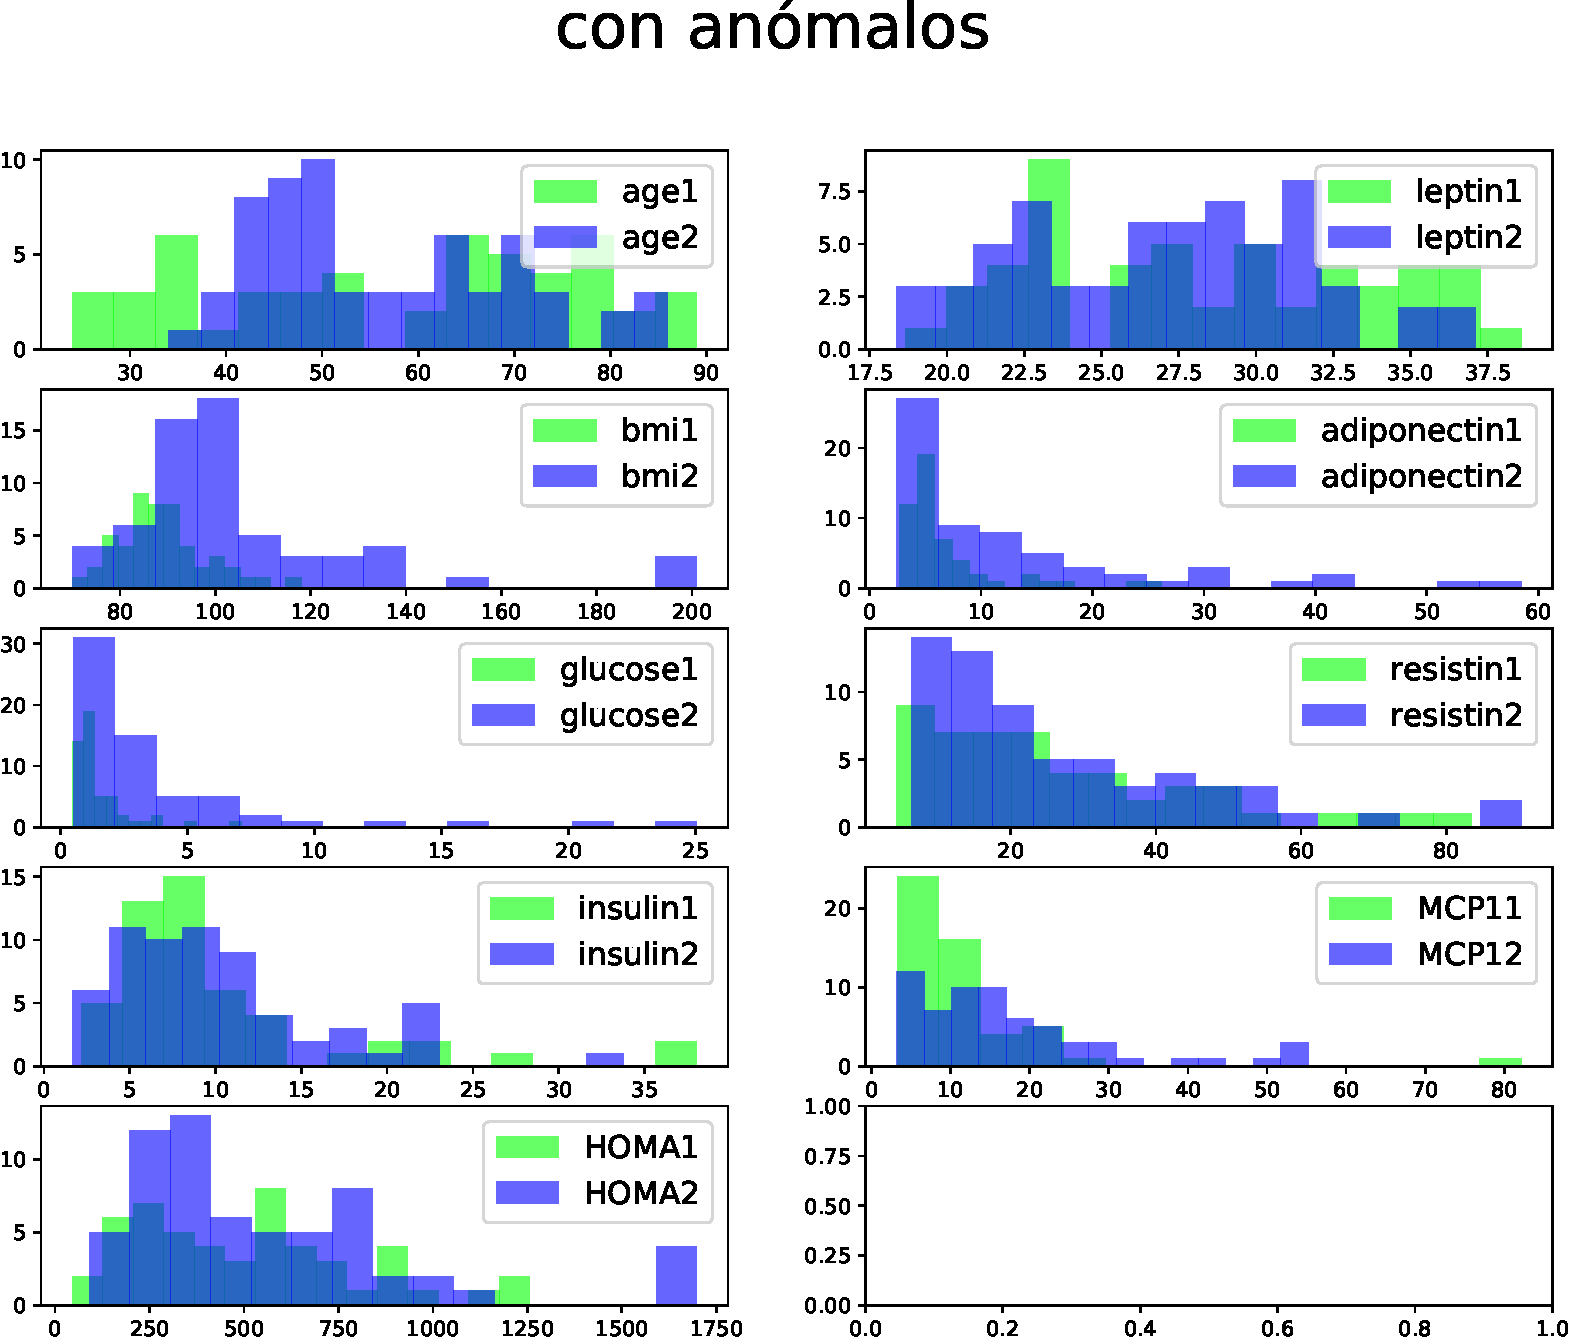
\includegraphics[width = 0.49\linewidth]{../python/images/hist.pdf}
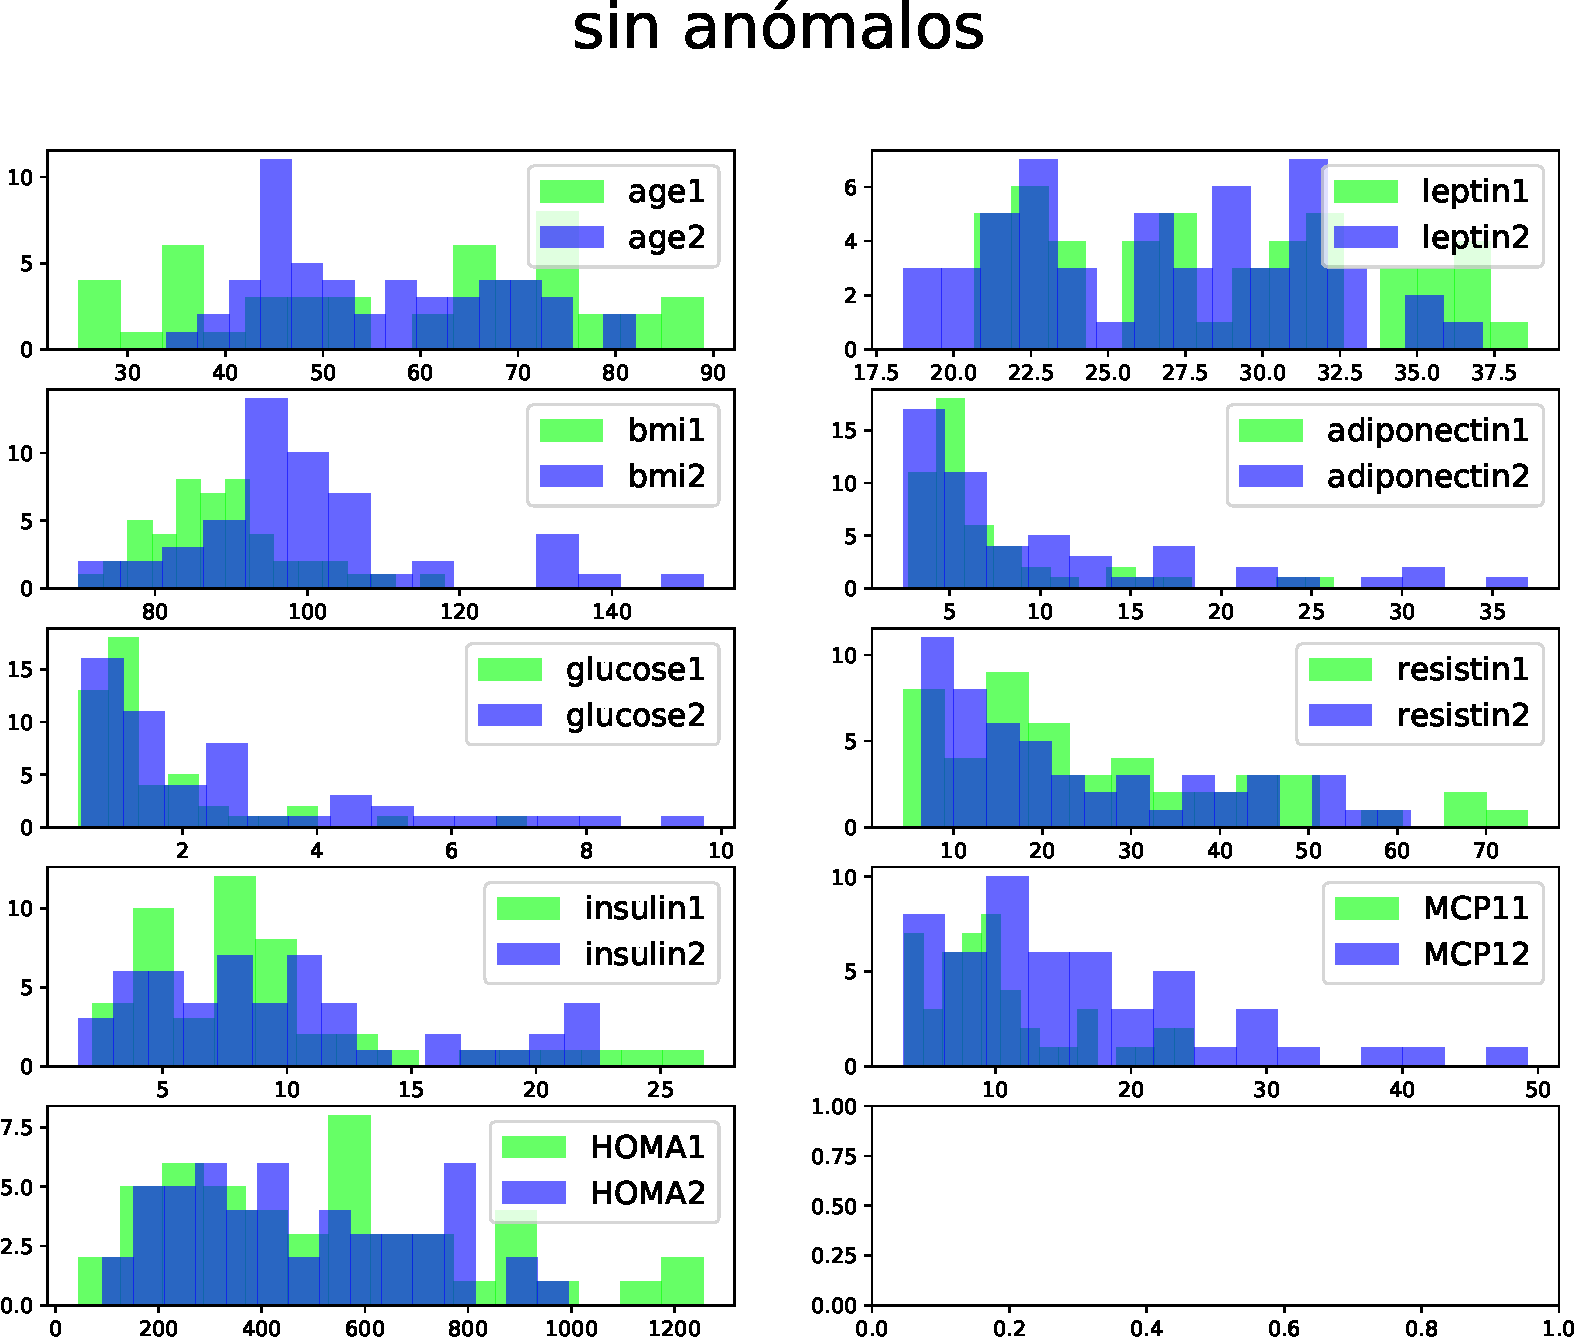
\includegraphics[width = 0.49\linewidth]{../python/images/hist1.pdf}
\caption{Histogramas para datos con y sin anomalias.}
\label{fig:hists}
\end{figure}

\lstinputlisting[
	linerange = {9-30},
	caption = {C\'odigo generador de los histogramas con datos
	an\'omalos.},
	]{../python/src/histograms.py}

\section{Kernel Density}

\begin{figure}[h]
\centering
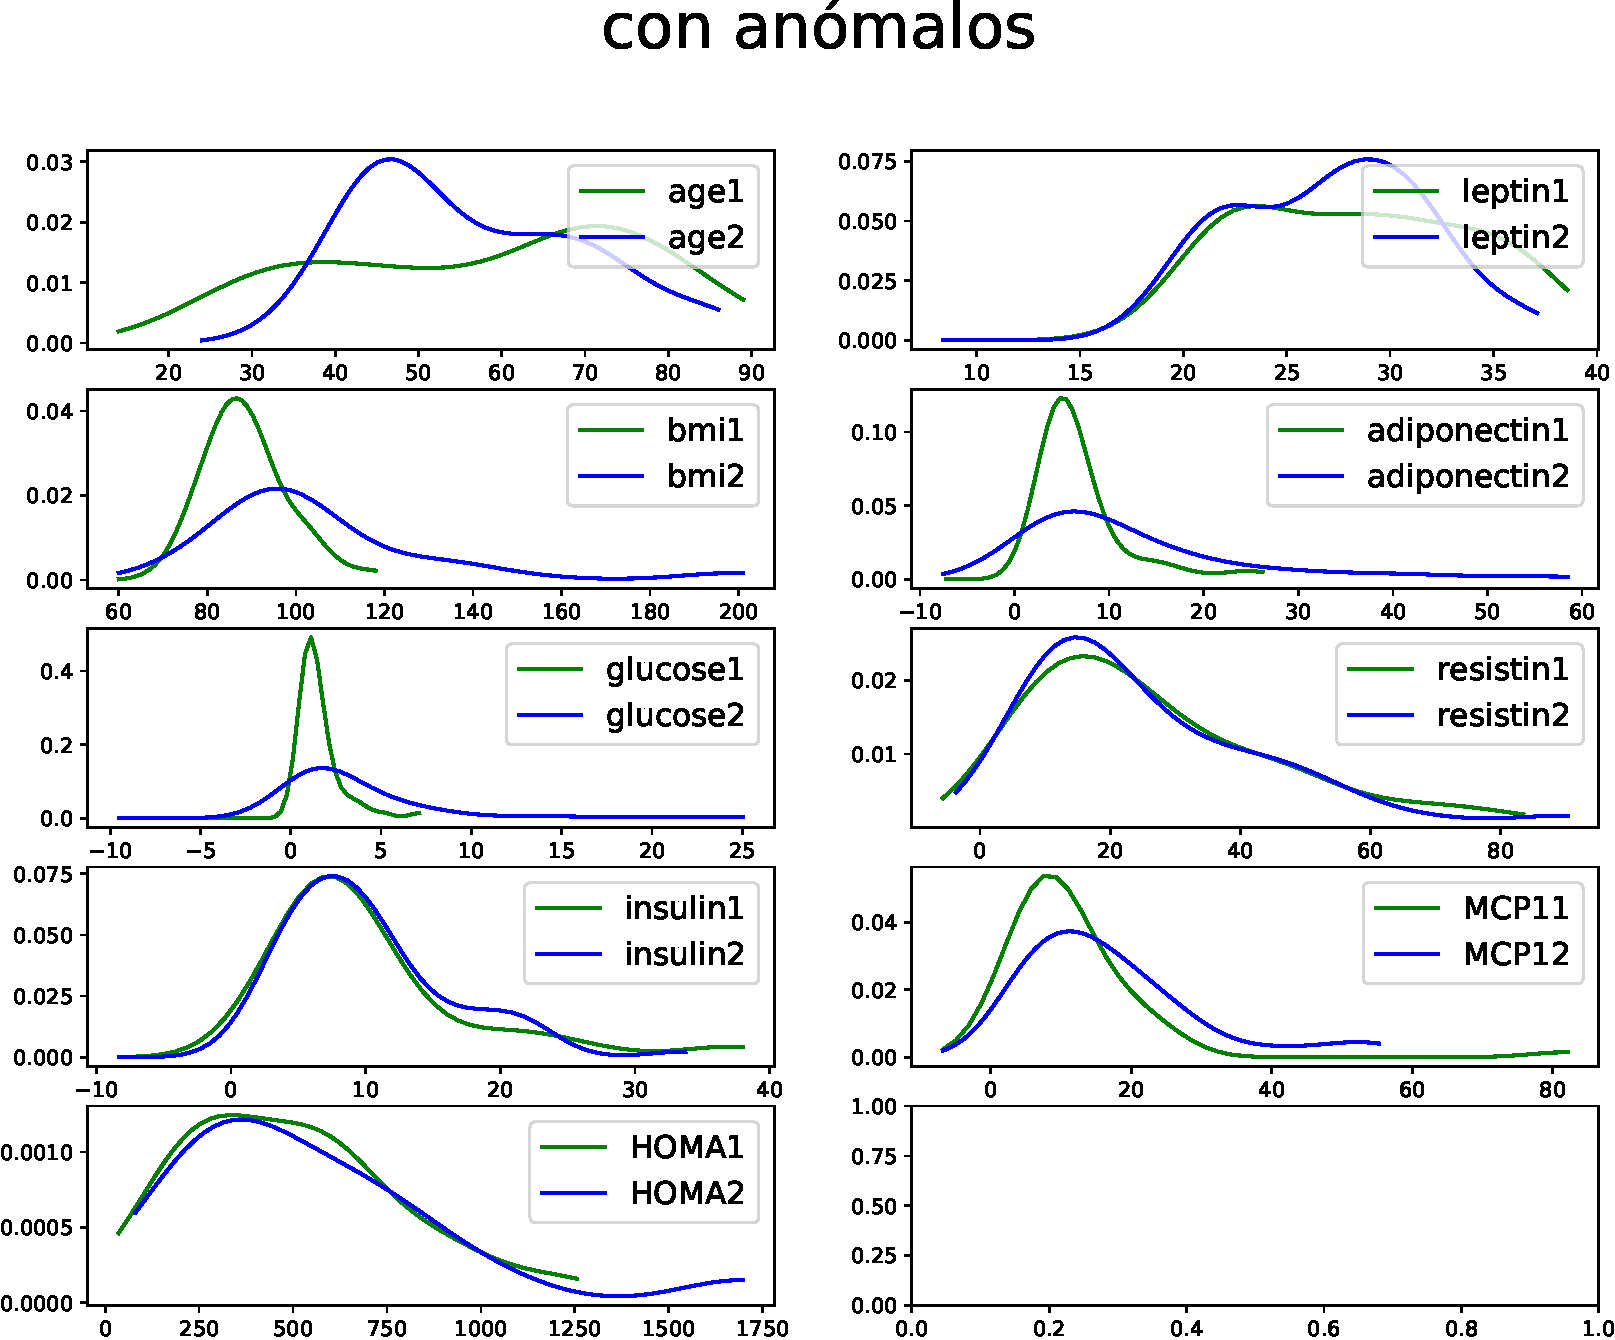
\includegraphics[width = 0.49\linewidth]{../python/images/kden.pdf}
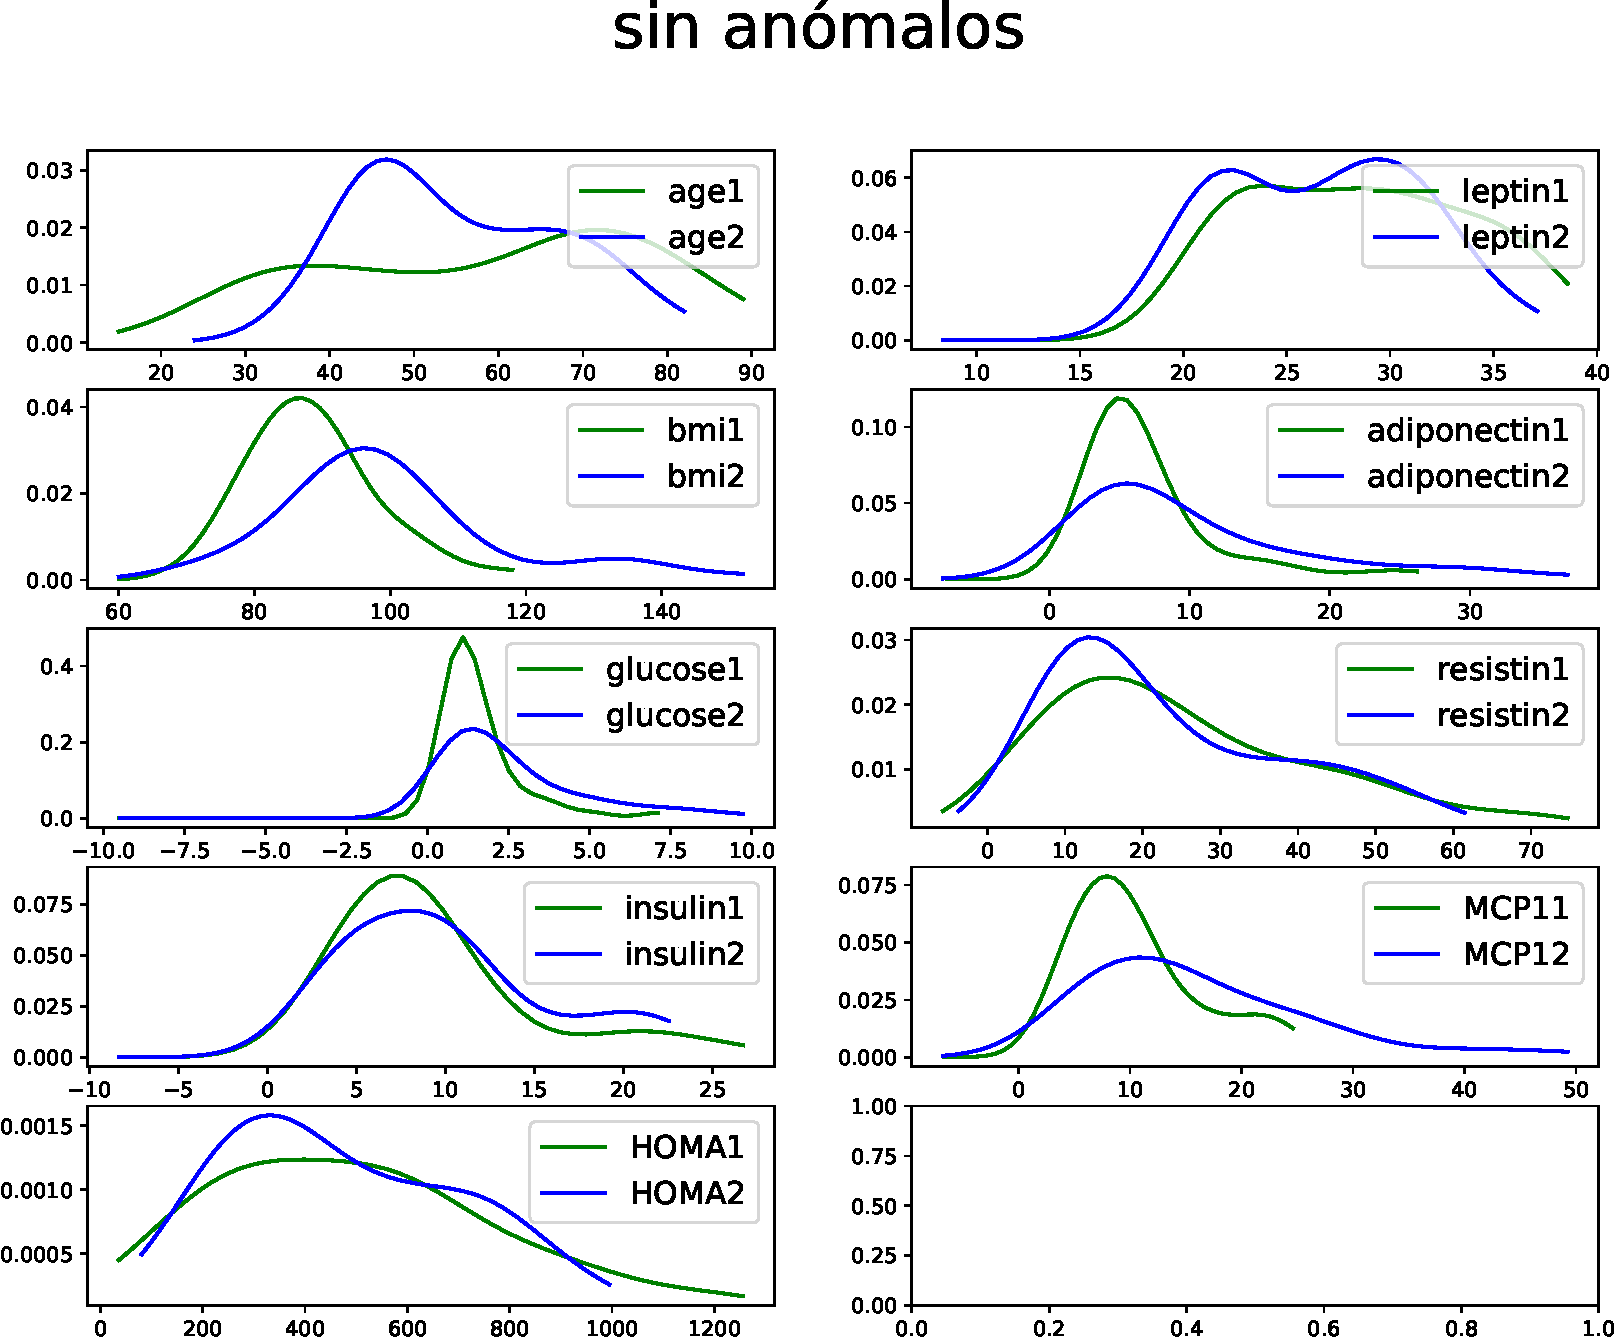
\includegraphics[width = 0.49\linewidth]{../python/images/kden1.pdf}
\caption{Kernel Density para datos con y sin anomalias.}
\label{fig:kdens}
\end{figure}

\lstinputlisting[
	linerange = {9-32},
	caption = {C\'odigo generador de los kernel density plots con datos
	an\'omalos.},
	]{../python/src/kerneldensity.py}

\section{Boxplot}

\begin{figure}[h]
\centering
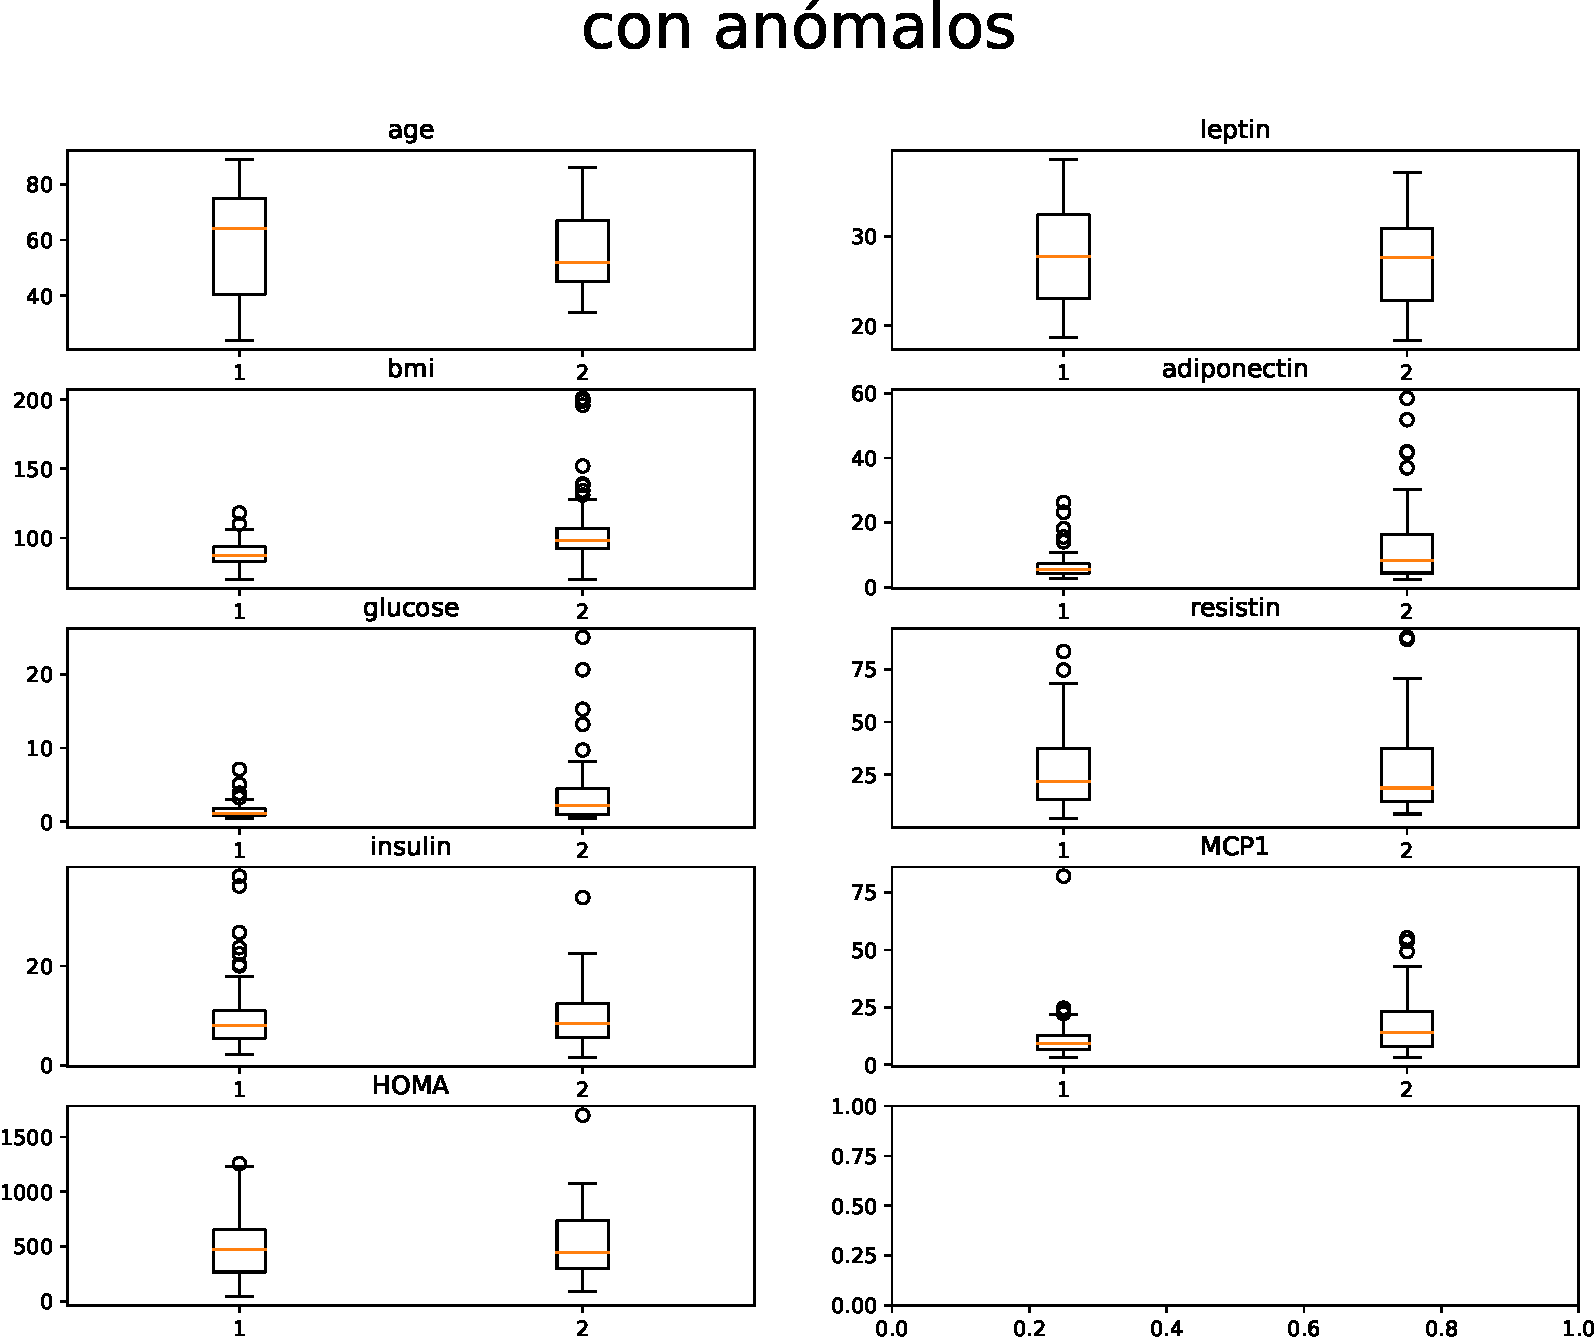
\includegraphics[width = 0.49\linewidth]{../python/images/boxp.pdf}
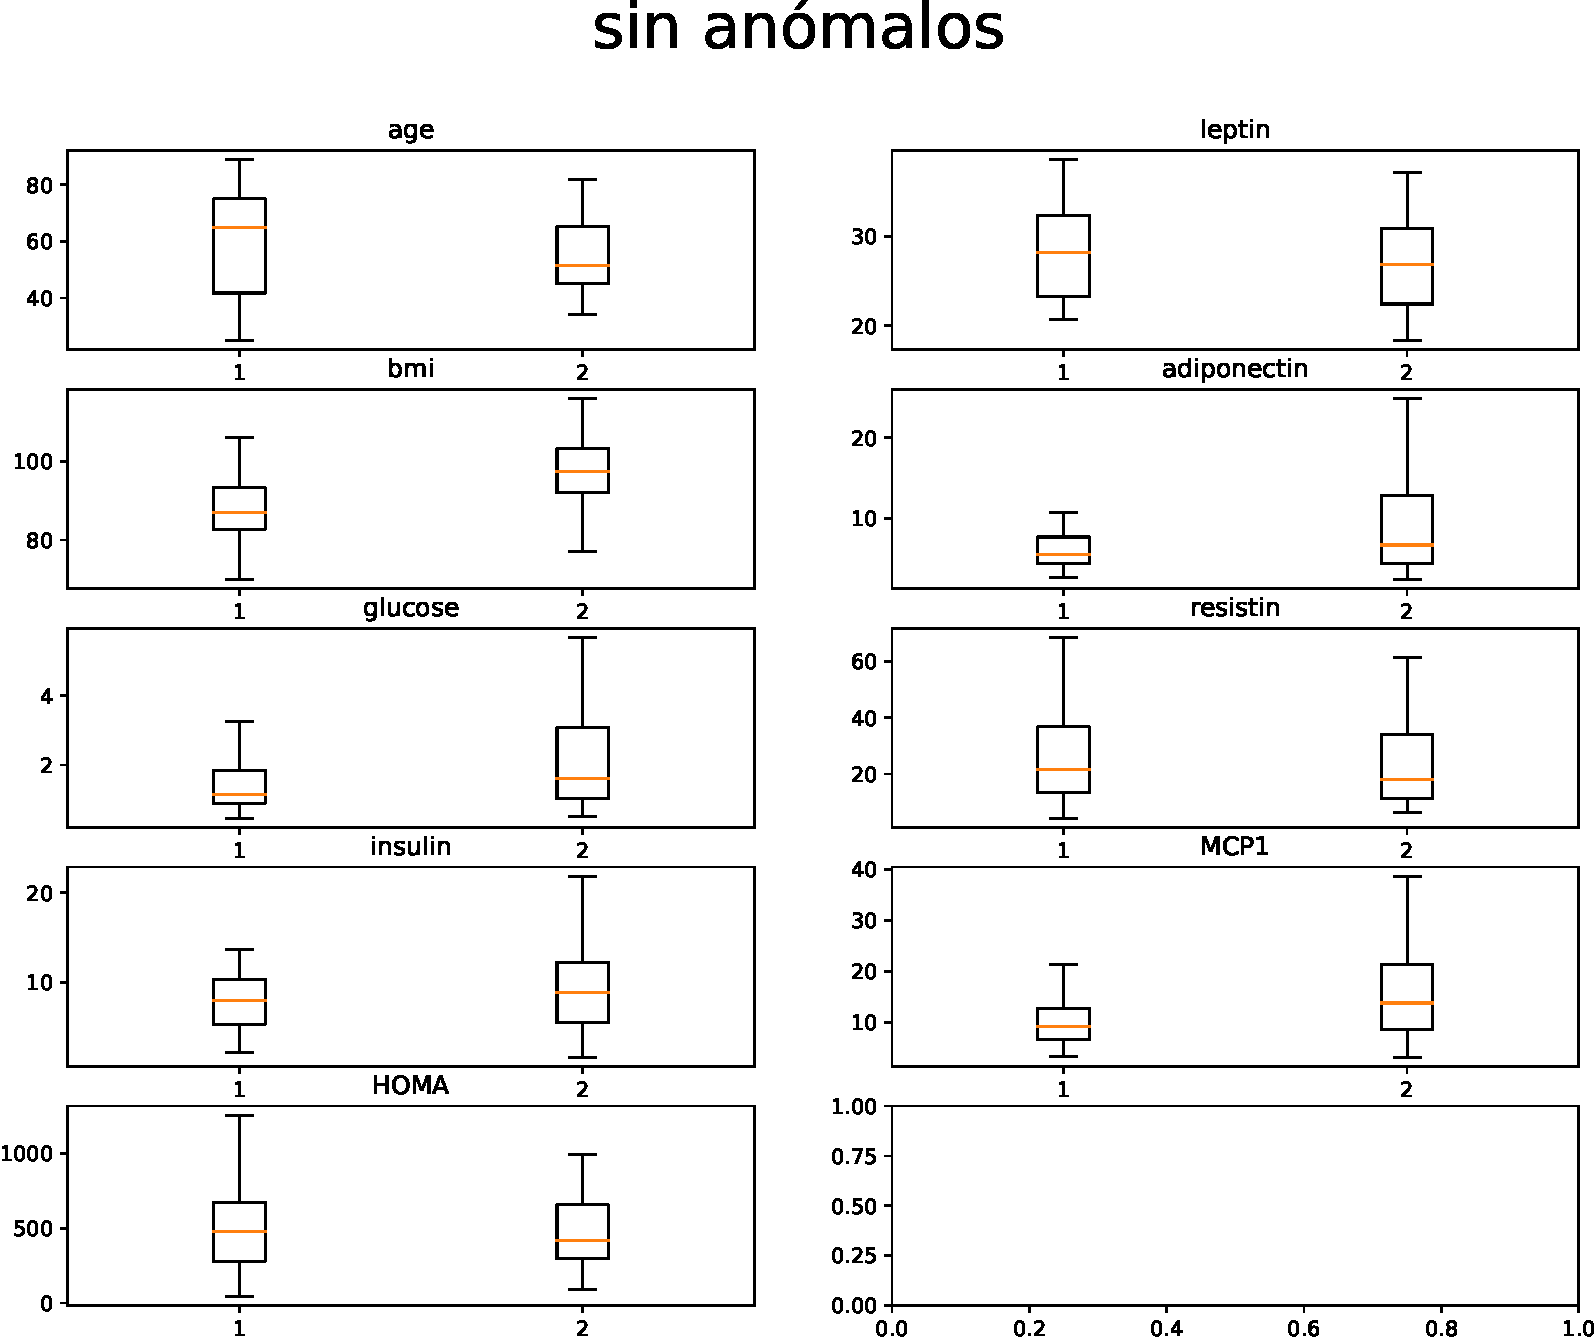
\includegraphics[width = 0.49\linewidth]{../python/images/boxp1.pdf}
\caption{Boxplots para datos con y sin anomalias.}
\label{fig:boxps}
\end{figure}

\lstinputlisting[
	linerange = {9-24},
	caption = {C\'odigo generador de los boxplots con datos
	an\'omalos.},
	]{../python/src/boxplot.py}

\newpage
\section{QQplot}

\begin{figure}[h]
\centering
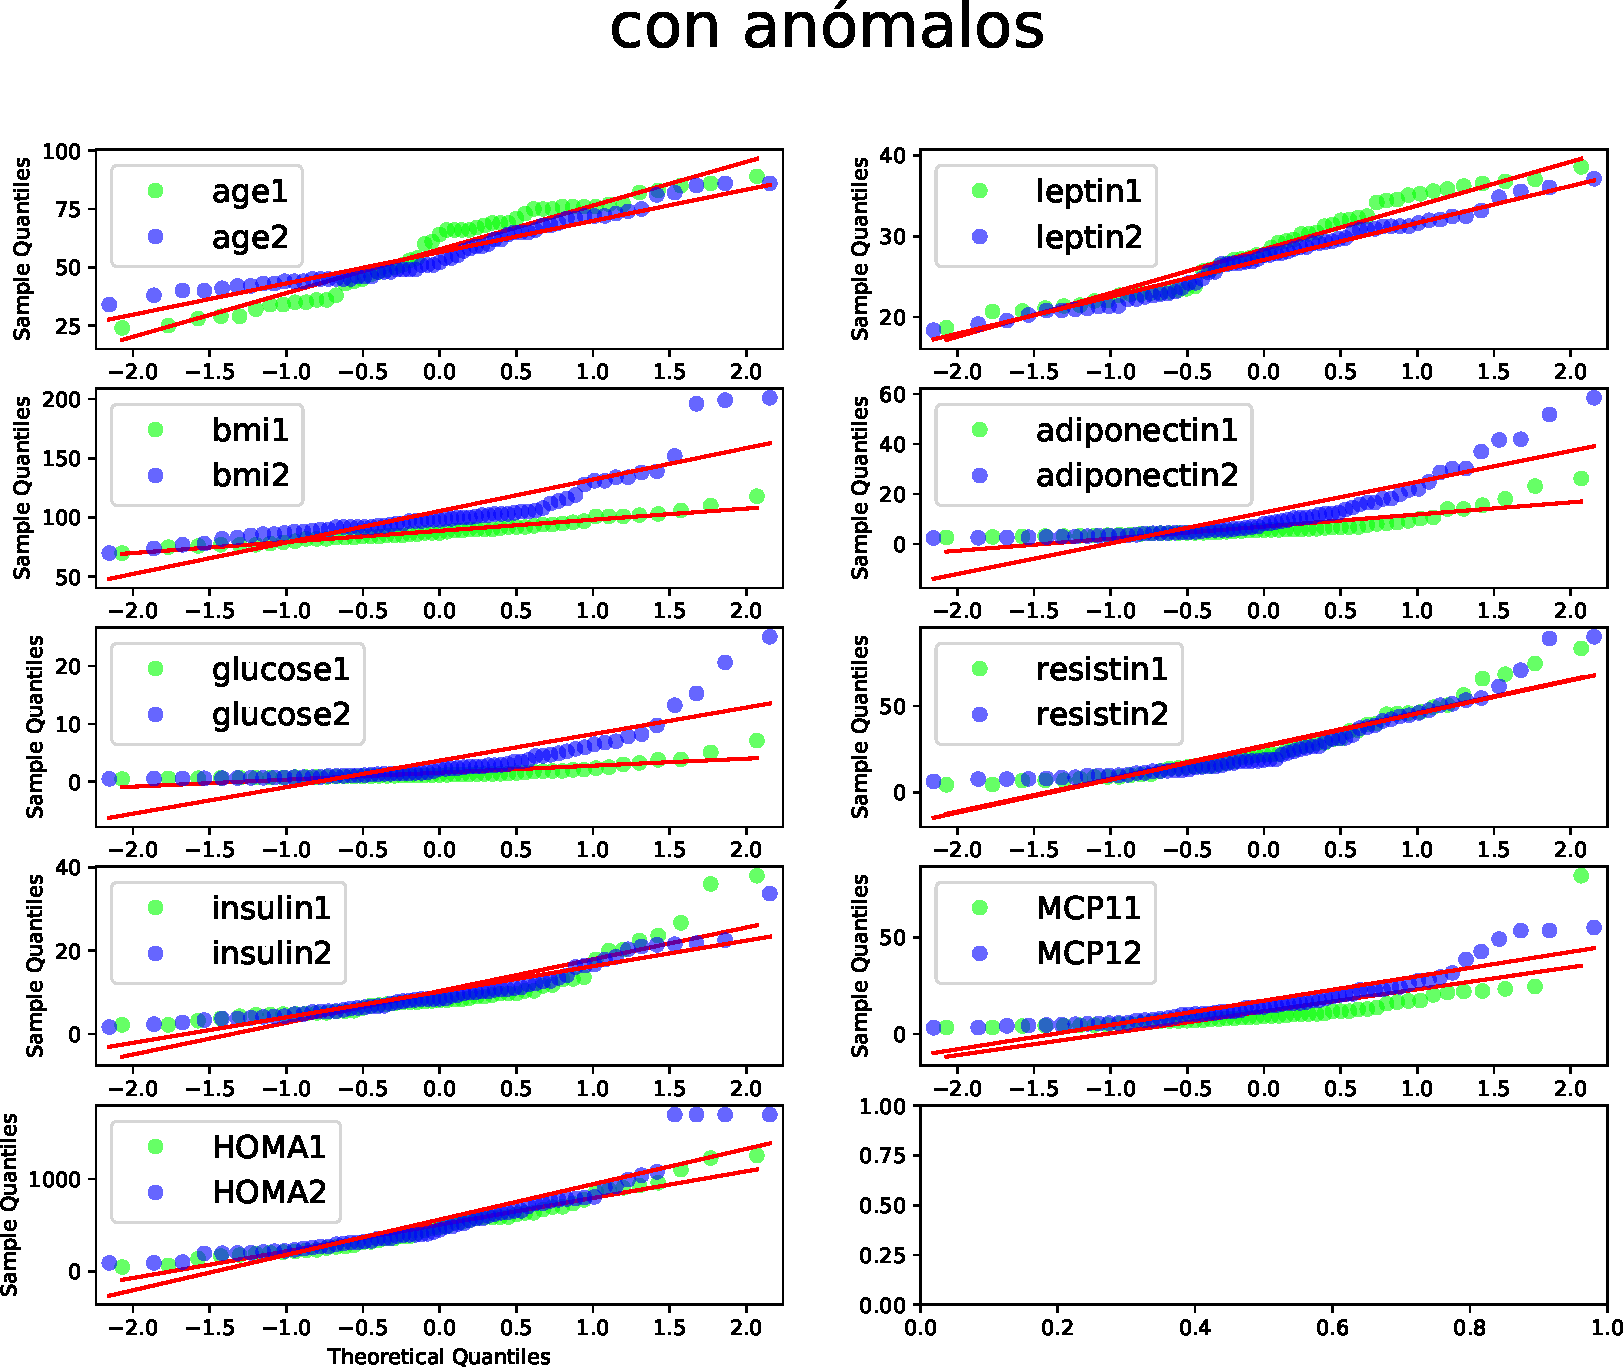
\includegraphics[width = 0.49\linewidth]{../python/images/qqp.pdf}
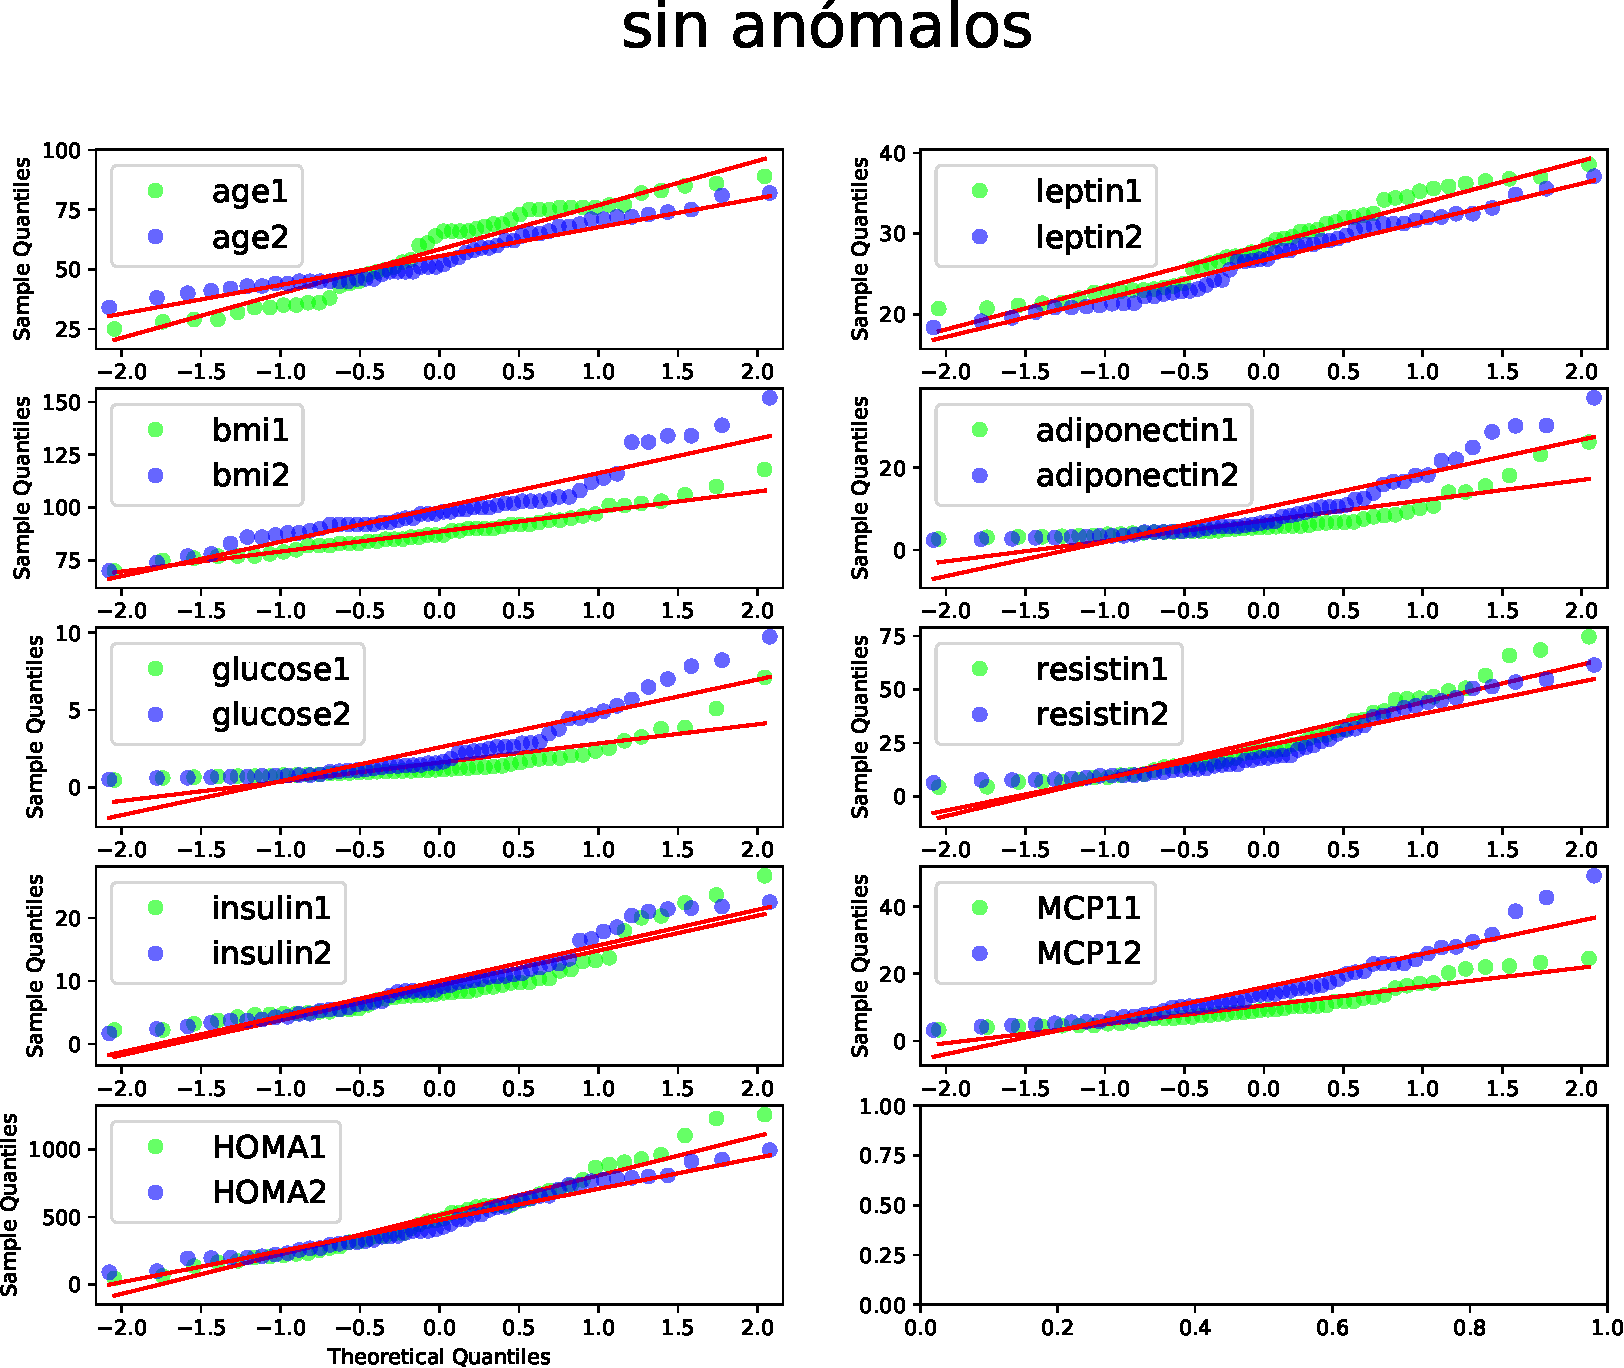
\includegraphics[width = 0.49\linewidth]{../python/images/qqp1.pdf}
\caption{QQplots para datos con y sin anomalias.}
\label{fig:qqps}
\end{figure}

\lstinputlisting[
	linerange = {9-28},
	caption = {C\'odigo generador de los QQplots con datos
	an\'omalos.},
	]{../python/src/qqplot.py}

\newpage
\section{Corrplot}

\begin{figure}[h]
\centering
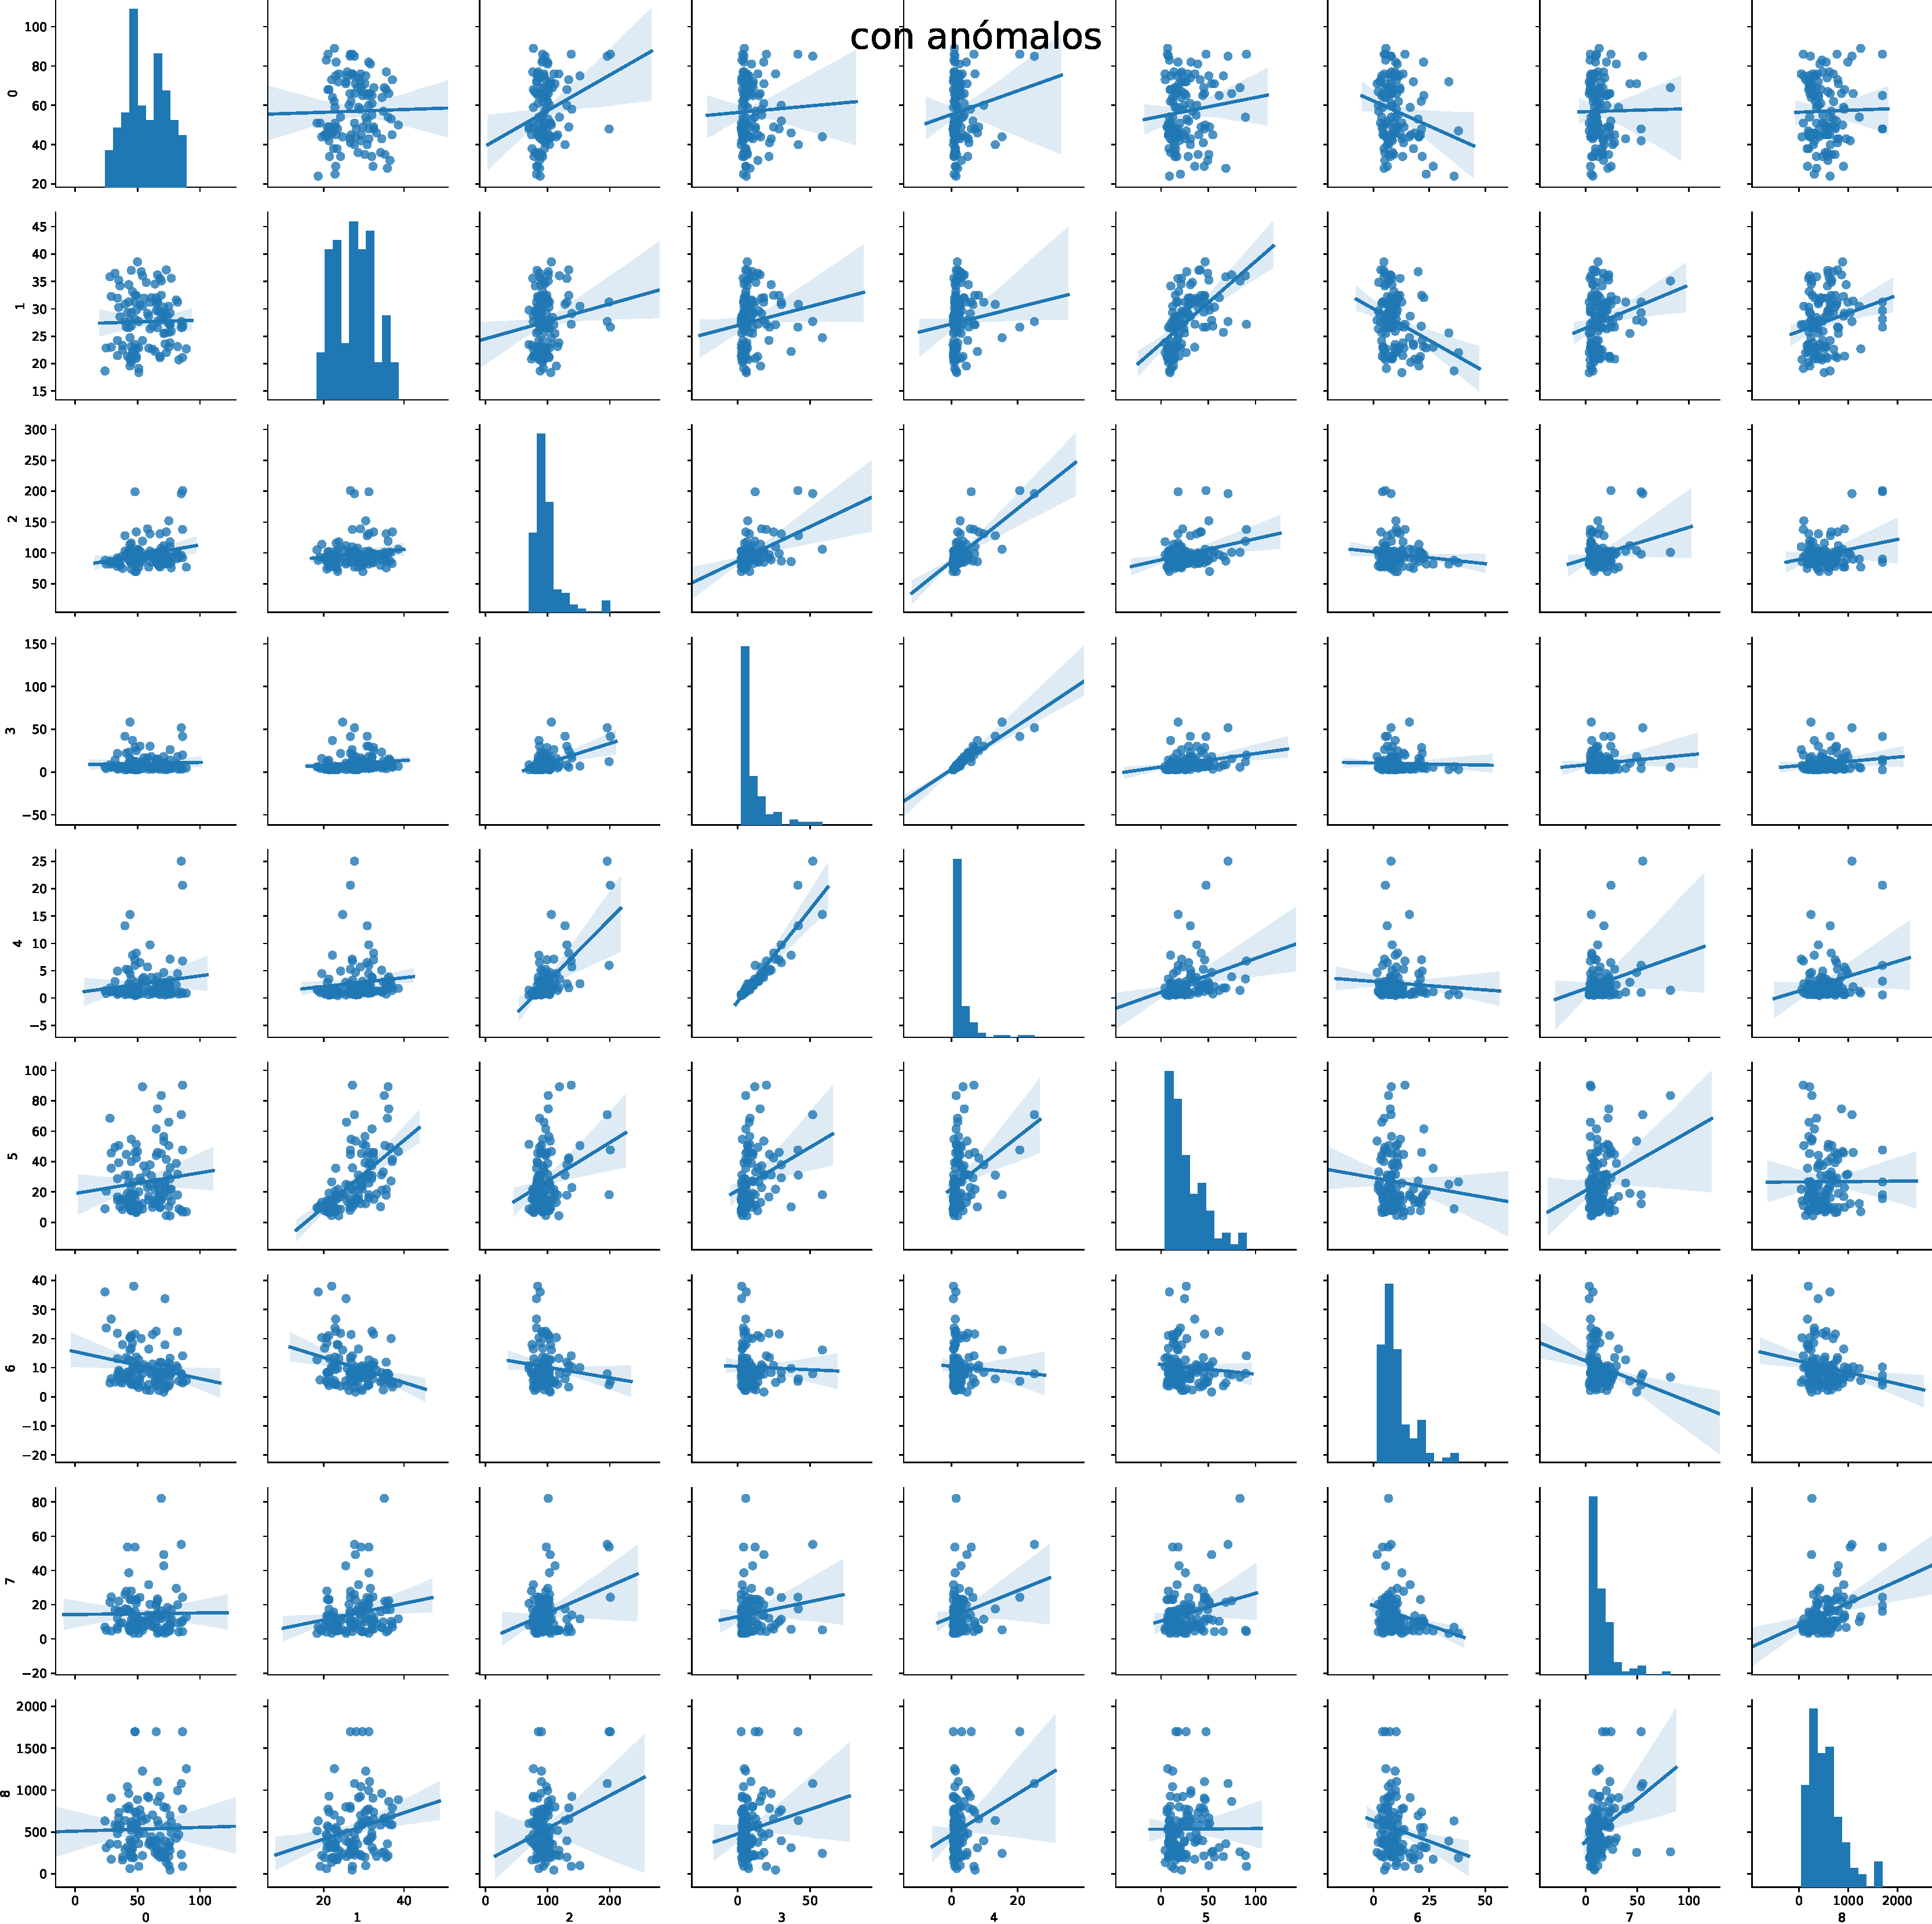
\includegraphics[width = \linewidth]{../python/images/corrp.pdf}
\caption{Corrplot para datos con anomalias.}
\label{fig:cps}
\end{figure}

\lstinputlisting[
	linerange = {11-18},
	caption = {C\'odigo generador de los corrplots con datos
	an\'omalos.},
	]{../python/src/corrplot.py}

\begin{figure}[h]
\centering
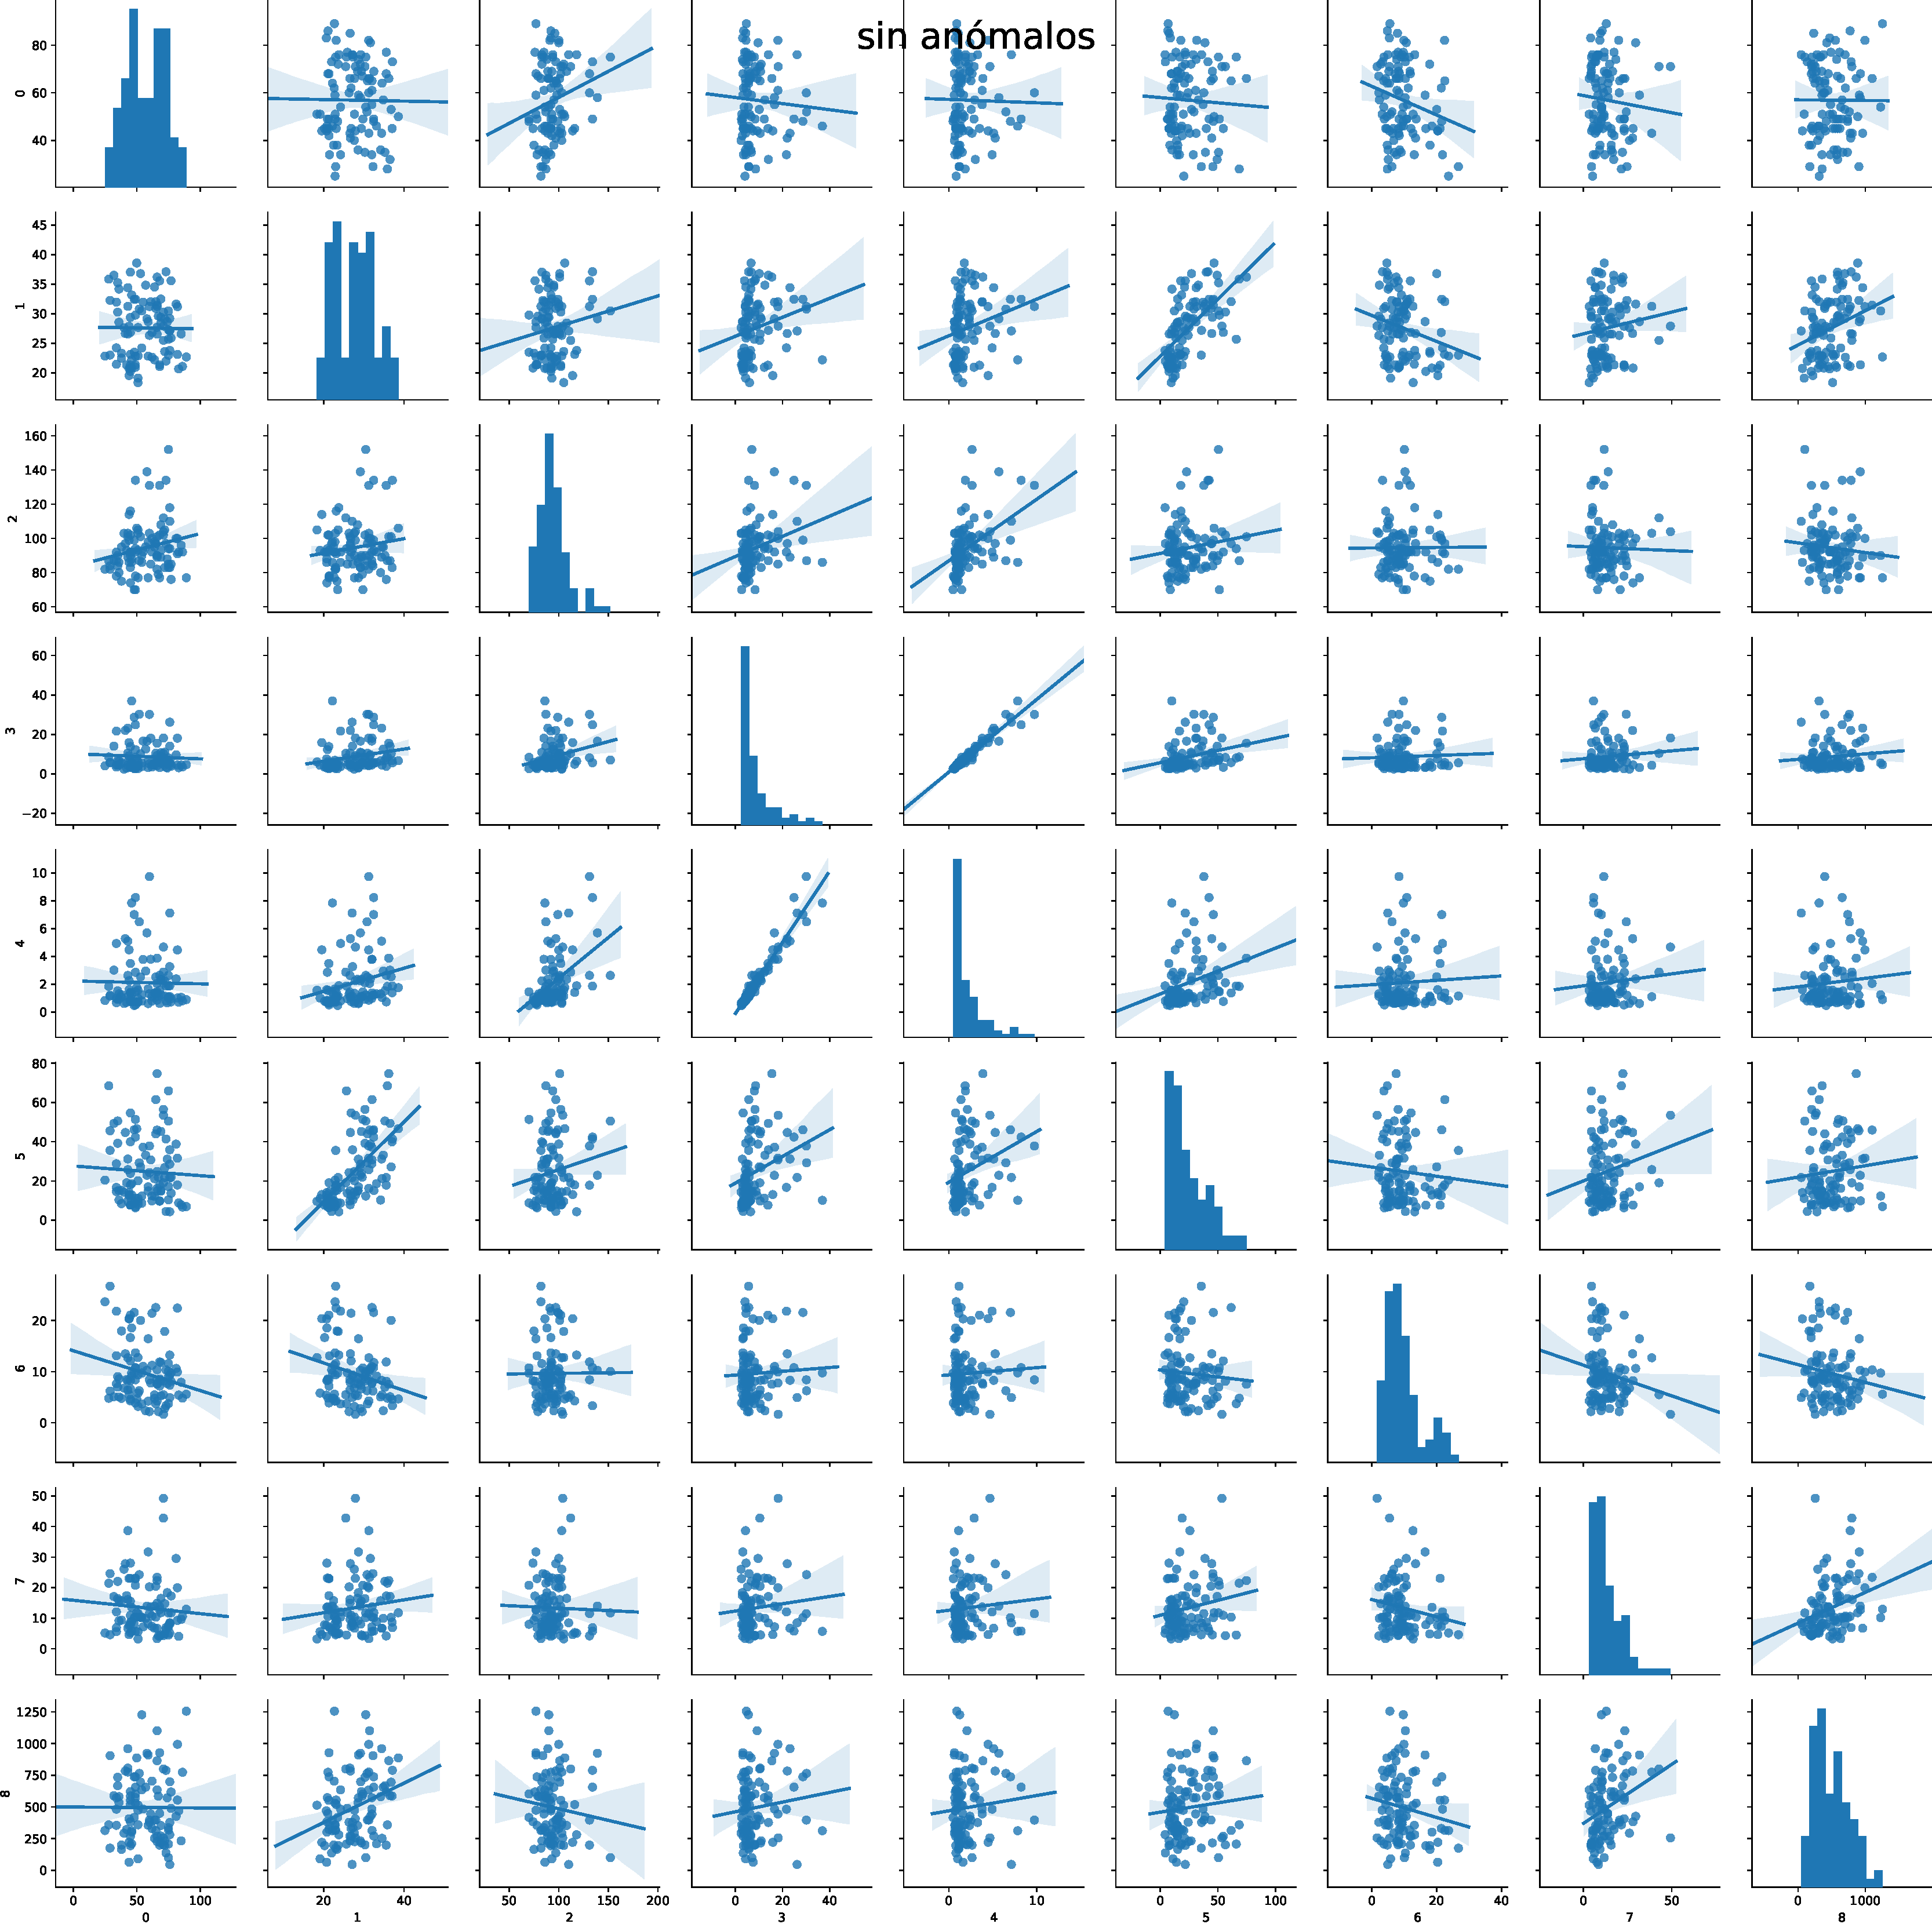
\includegraphics[width = \linewidth]{../python/images/corrp1.pdf}
\caption{Corrplot para datos sin anomalias.}
\label{fig:cp1s}
\end{figure}

\end{document}
